\documentclass[handout]{beamer}
%\documentclass{beamer}
\usepackage{tikz}
\usetikzlibrary{positioning}
\usepackage[normalem]{ulem}
\usepackage{xcolor}
\usepackage{array}
\usepackage[backend=biber,citestyle=authoryear]{biblatex}
\addbibresource{ref.bib}

\usepackage{makecell}

\renewcommand\theadalign{bc}
\renewcommand\theadfont{\bfseries}
\renewcommand\theadgape{\Gape[4pt]}
\renewcommand\cellgape{\Gape[4pt]}


\tikzstyle{every picture}+=[remember picture]
\usetikzlibrary{positioning}
\usetikzlibrary{decorations.pathreplacing}

\usetheme{CambridgeUS}
\graphicspath{{figures/}}
\newcommand{\bvar}[1]{\mathbf{#1}} 
\definecolor{red}{HTML}{cf161e}
\definecolor{lgrey}{HTML}{dddddd}
\definecolor{bgray}{HTML}{E8E6E2}
\makeatletter
\setbeamertemplate{footline}
{
  \leavevmode%
  \hbox{%
  \begin{beamercolorbox}[wd=.5\paperwidth,ht=2.25ex,dp=1ex,center]{author in head/foot}%
    \usebeamerfont{author in head/foot}\insertshortauthor~~\beamer@ifempty{\insertshortinstitute}{}{(\insertshortinstitute)}
  \end{beamercolorbox}%
  \begin{beamercolorbox}[wd=.5\paperwidth,ht=2.25ex,dp=1ex,center]{date in head/foot}%
    \usebeamerfont{date in head/foot}\insertshorttitle{}
  \end{beamercolorbox}}%
  \vskip0pt%
}
\makeatother
   
\setbeamercolor{normal text}{fg=black,bg=white}
\setbeamercolor{block title}{bg=red,fg=white}
\setbeamercolor{block body}{bg=lgrey}
\setbeamercolor*{item}{fg=red}
\setbeamercolor{structure}{fg=red}
\setbeamercolor{background canvas}{parent=normal text}
\setbeamercolor{background}{parent=background canvas}
\setbeamercolor{frametitle}{fg=red}
\setbeamercolor{section in head/foot}{bg=red}
\setbeamercolor{author in head/foot}{bg=red}
\setbeamercolor{date in head/foot}{fg=red}


\title{\textcolor{red}{Bias-Variance Tradeoffs in Joint Spectral Embeddings}}
\author[Benjamin Draves]{Benjamin Draves \and Daniel Sussman}
\institute[Boston Univeristy] 
{\normalsize Boston University}

\date{Joint Statistical Meetings, 1 August 2020}

\begin{document}

\begin{frame}
  \titlepage
\end{frame}

%--------------------------------------------------------------
\section{Joint Network Embeddings}

\begin{frame}{Multiplex Networks}
\begin{itemize}
    \item Multiplex networks encode multiple relationships between entities as a collection of networks. 
    \begin{center}
        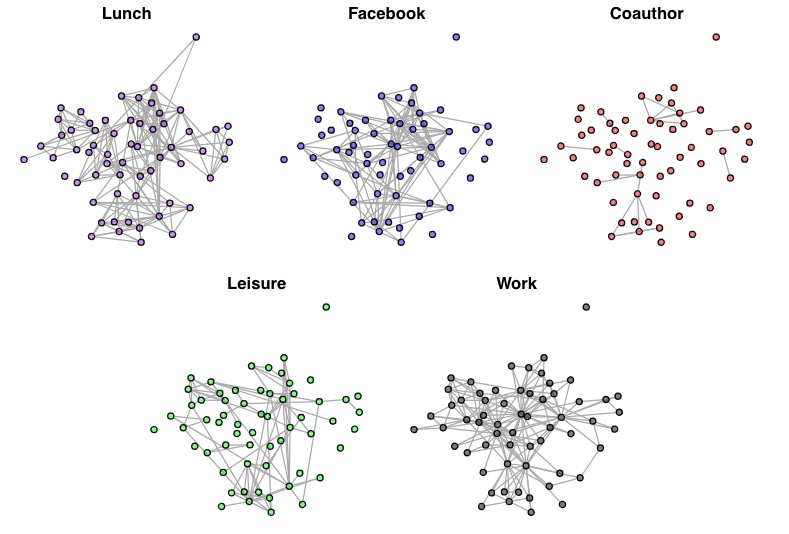
\includegraphics[width=0.6\textwidth]{aarhus_multiplex.jpg}
    \end{center}\pause
    \item Application areas; International Trade, Transportation Systems, Terrorist Groups, Neuroscience \parencite{Kivela2014}. 
\end{itemize}
\end{frame}

\begin{frame}{Individual Spectral Embeddings}
\begin{center}
    \begin{tikzpicture}
    %Draw Networks
    \node[shape=rectangle, align = center] (G1) at (-4,2.5) {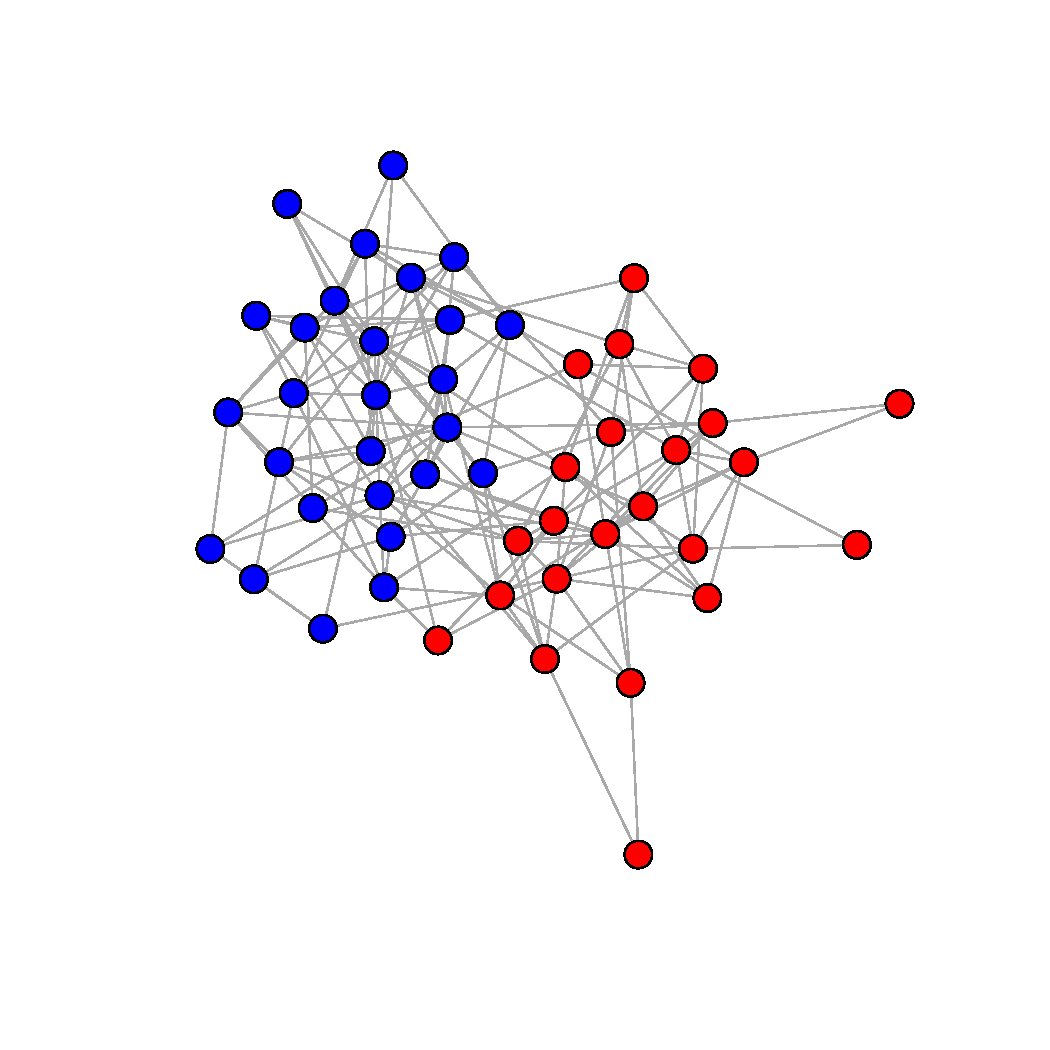
\includegraphics[width = 1in, height = 1in]{g1_beamer.pdf}};
    \node[shape=rectangle, align = center] (Gg) at (-4,0) {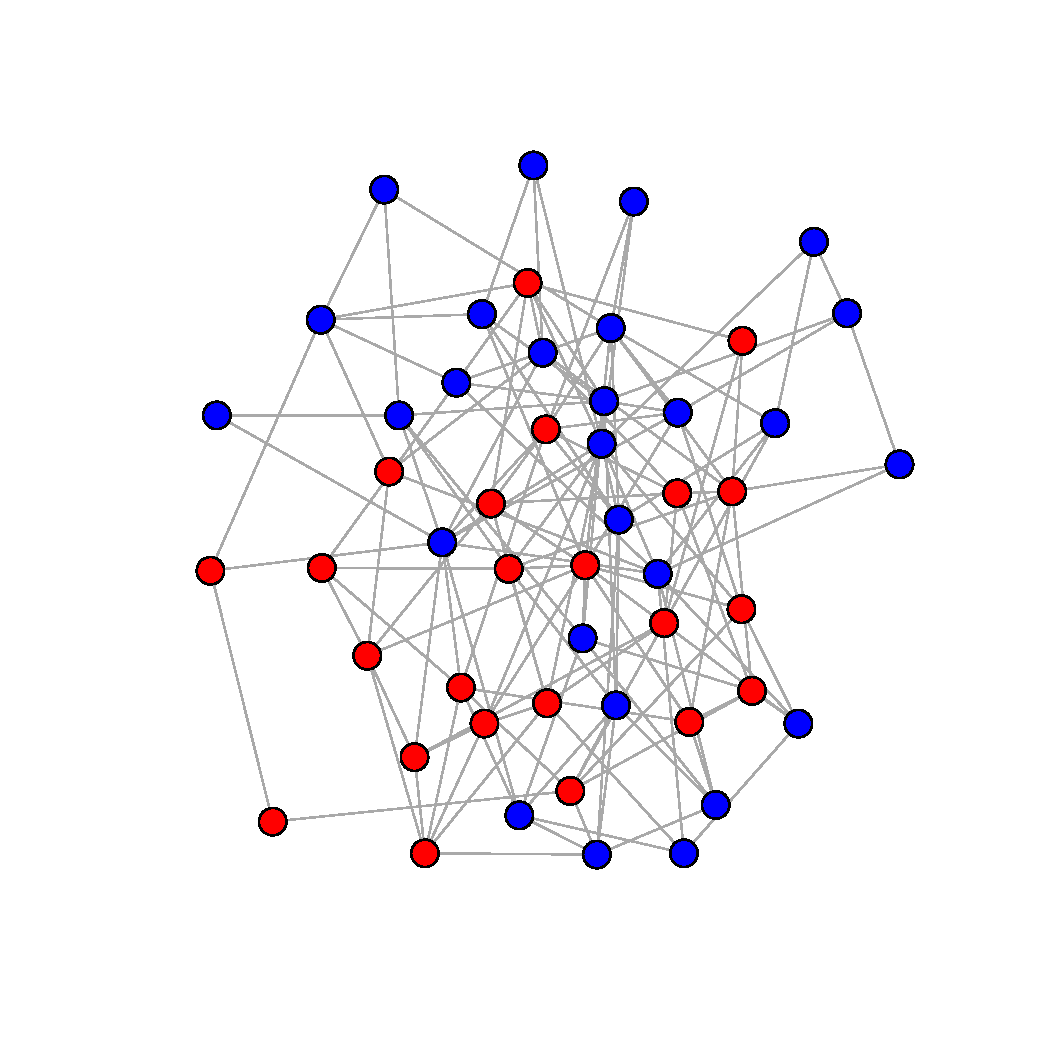
\includegraphics[width = 1in, height = 1in]{g2_beamer.pdf}};
    \node[shape=rectangle, align = center] (Gm) at (-4,-2.5) {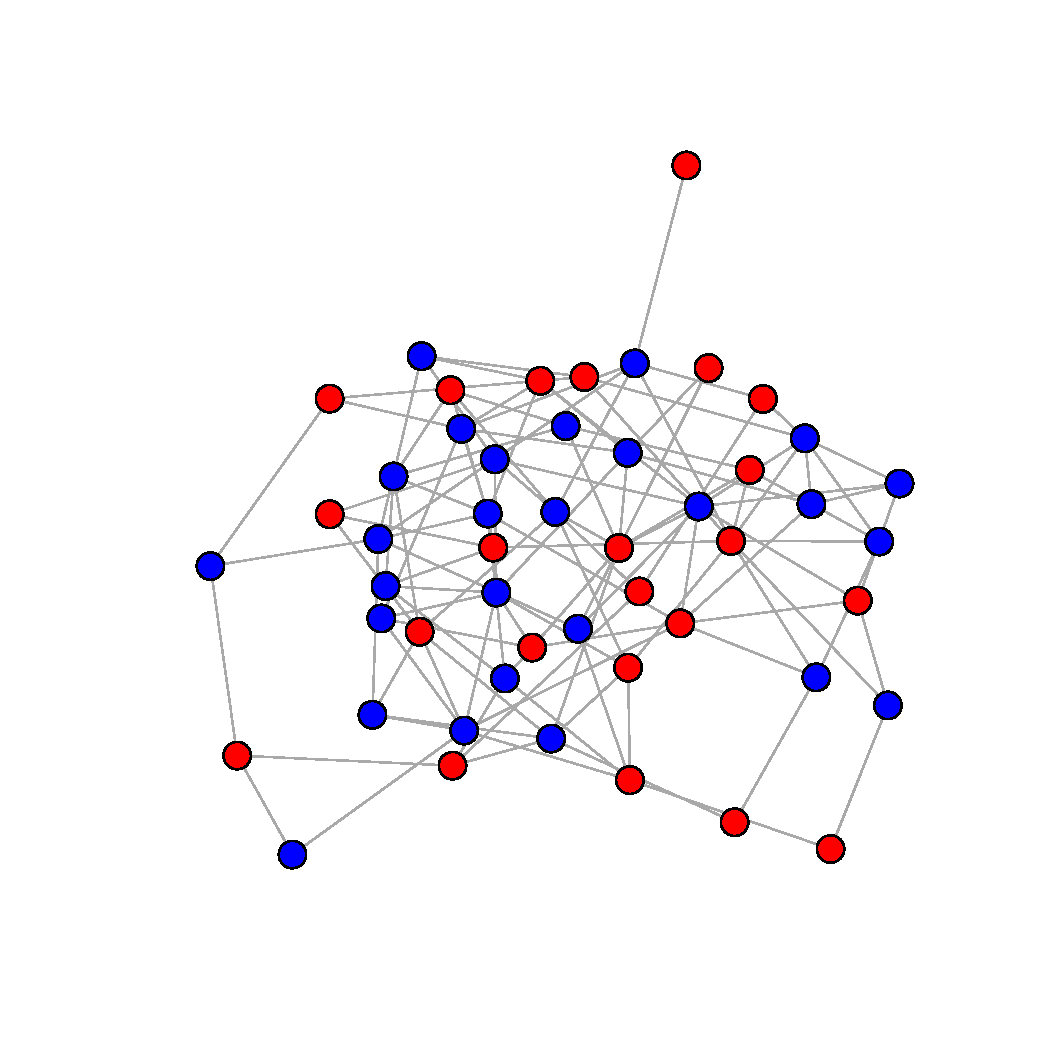
\includegraphics[width = 1in, height = 1in]{g3_beamer.pdf}};
    
    %Draw Adjacency Matrices
    \node[shape=rectangle, align = center] (A1) at (-2,2.5) {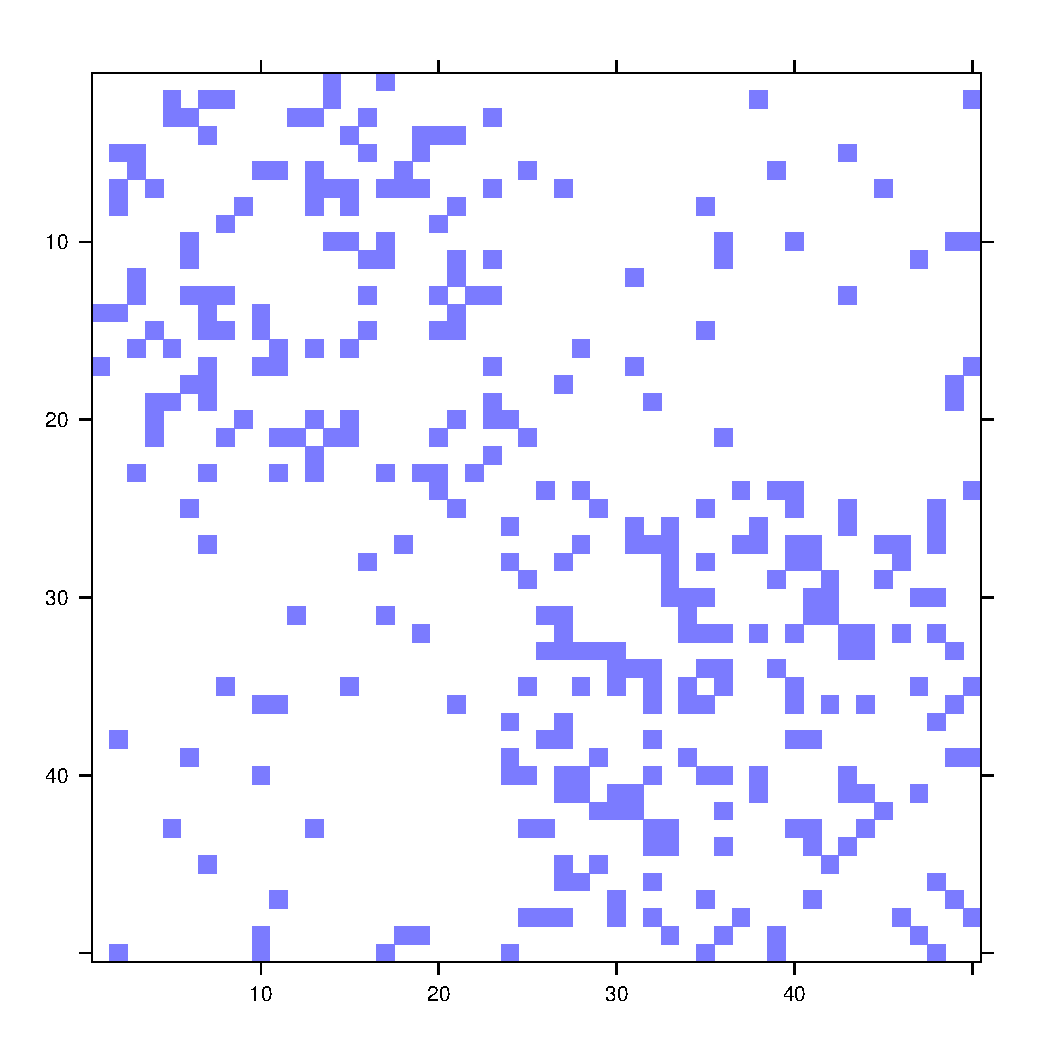
\includegraphics[width = .7in, height = .7in]{A1_beamer.pdf}};
    \node[shape=rectangle, align = center] (Ag) at (-2,0) {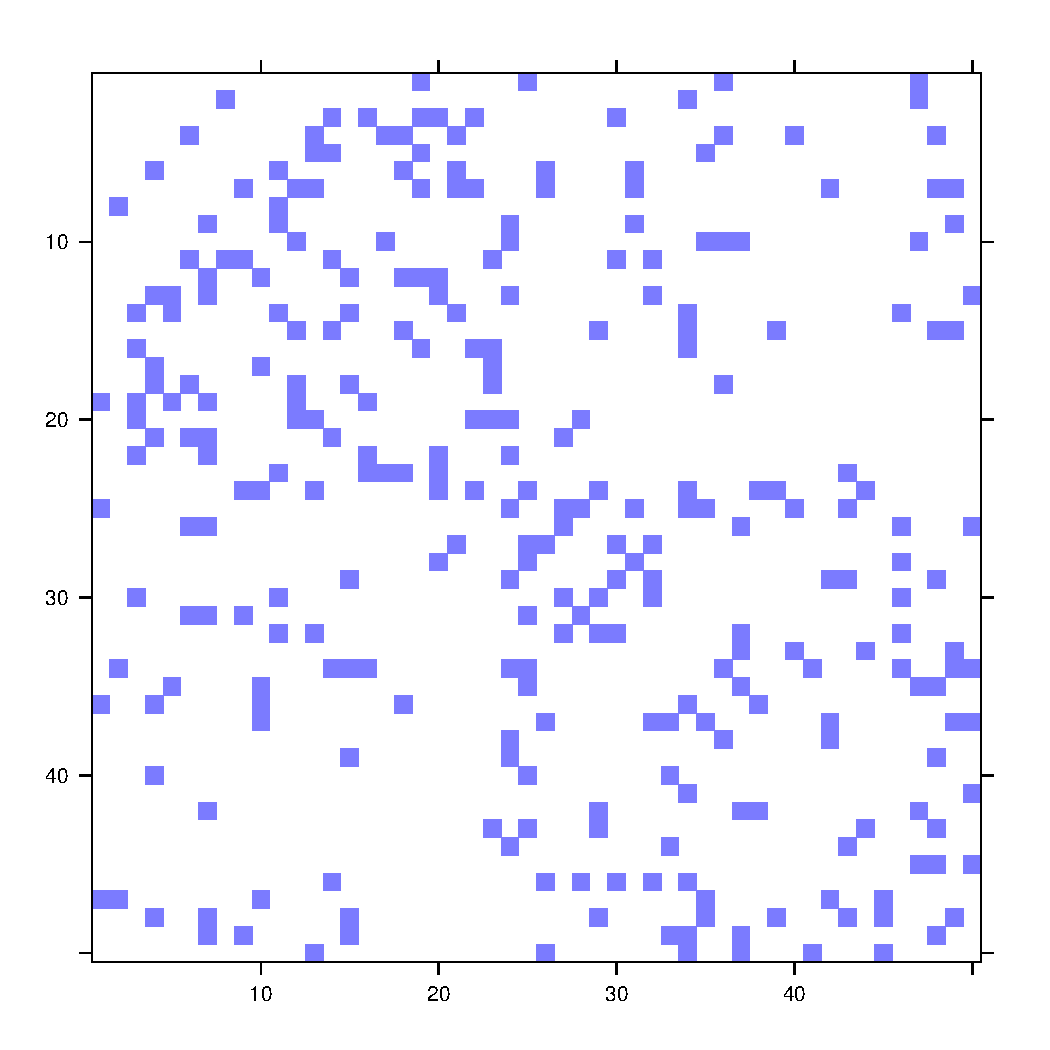
\includegraphics[width = .7in, height = .7in]{A2_beamer.pdf}};
    \node[shape=rectangle, align = center] (Am) at (-2,-2.5) {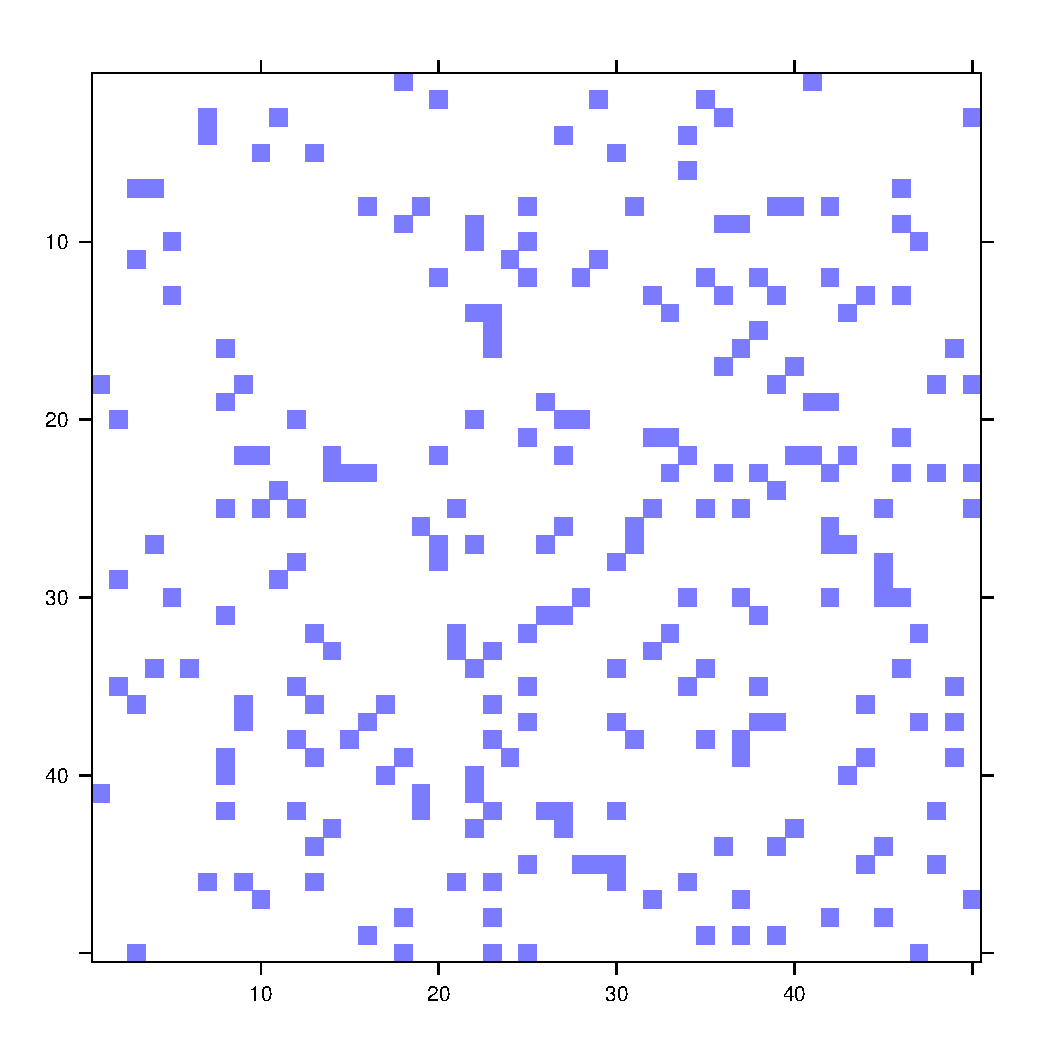
\includegraphics[width = .7in, height = .7in]{A3_beamer.pdf}};\pause
    
    
    %Draw ASE boxes
    \node[shape=rectangle, align = center, draw = black] (ASE1) at (.5, 2.5){\scriptsize{ASE}};
    \node[shape=rectangle, align = center, draw = black] (ASEg) at (.5, 0){\scriptsize{ASE}};
    \node[shape=rectangle, align = center, draw = black] (ASEm) at (.5, -2.5){\scriptsize{ASE}};
    
    %Draw ASE
    \node[shape=rectangle, align = center] (E1) at (3,2.5) {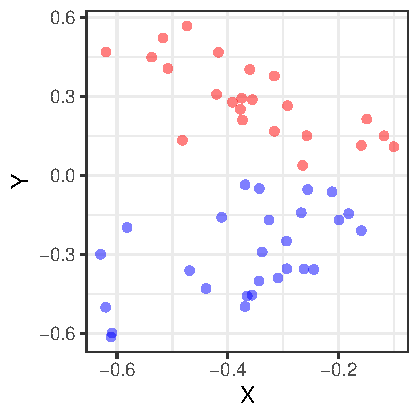
\includegraphics[width = .8in, height = .8in]{ase_0_three_vals.pdf}};
    \node[shape=rectangle, align = center] (Eg) at (3,0) {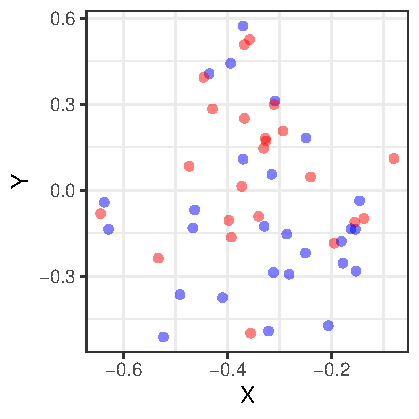
\includegraphics[width = 0.8in, height = .8in]{ase_5_three_vals.pdf}};
    \node[shape=rectangle, align = center] (Em) at (3,-2.5) {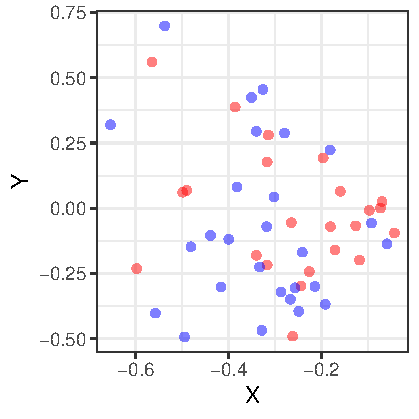
\includegraphics[width = 0.8in, height = .8in]{ase_1_three_vals.pdf}};
    
    %Draw arrows
    \draw (A1)--(ASE1); \draw[->] (ASE1)--(E1);
    \draw (Ag)--(ASEg); \draw[->] (ASEg)--(Eg);
    \draw (Am)--(ASEm); \draw[->] (ASEm)--(Em);
    \pause

    %draw bracket 
    \draw [decorate, decoration={brace,amplitude=10pt,raise=4pt}]
(4,3.5) -- (4,-3.5) node [black, midway, xshift=1.25cm, text width=1.5cm] {\footnotesize
Statistical Inference};
\end{tikzpicture}
\end{center}     
    
\end{frame}


\begin{frame}{Joint Spectral Embeddings}
\begin{center}
    \begin{tikzpicture}
    %Draw Networks
    \node[shape=rectangle, align = center] (G1) at (-4,2.5) {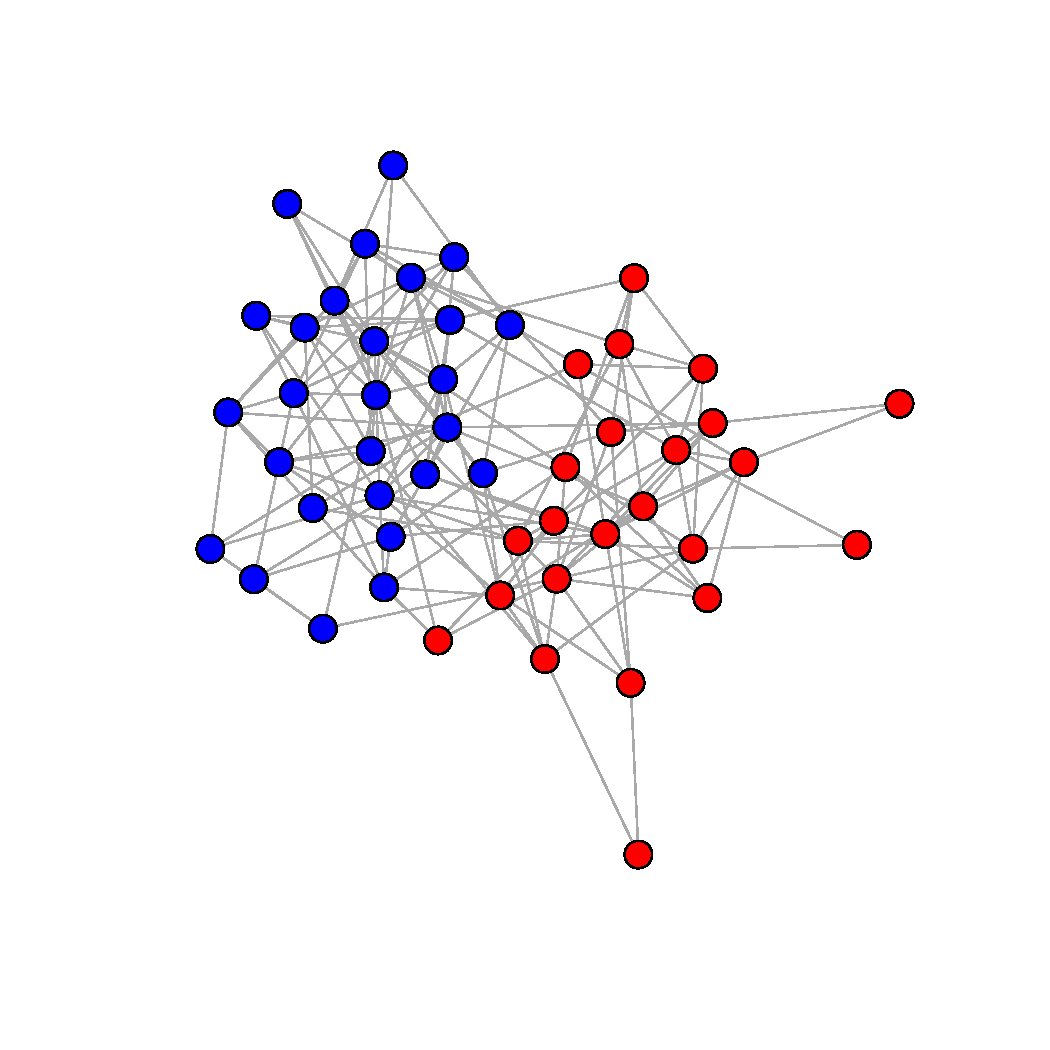
\includegraphics[width = 1in, height = 1in]{g1_beamer.pdf}};
    \node[shape=rectangle, align = center] (Gg) at (-4,0) {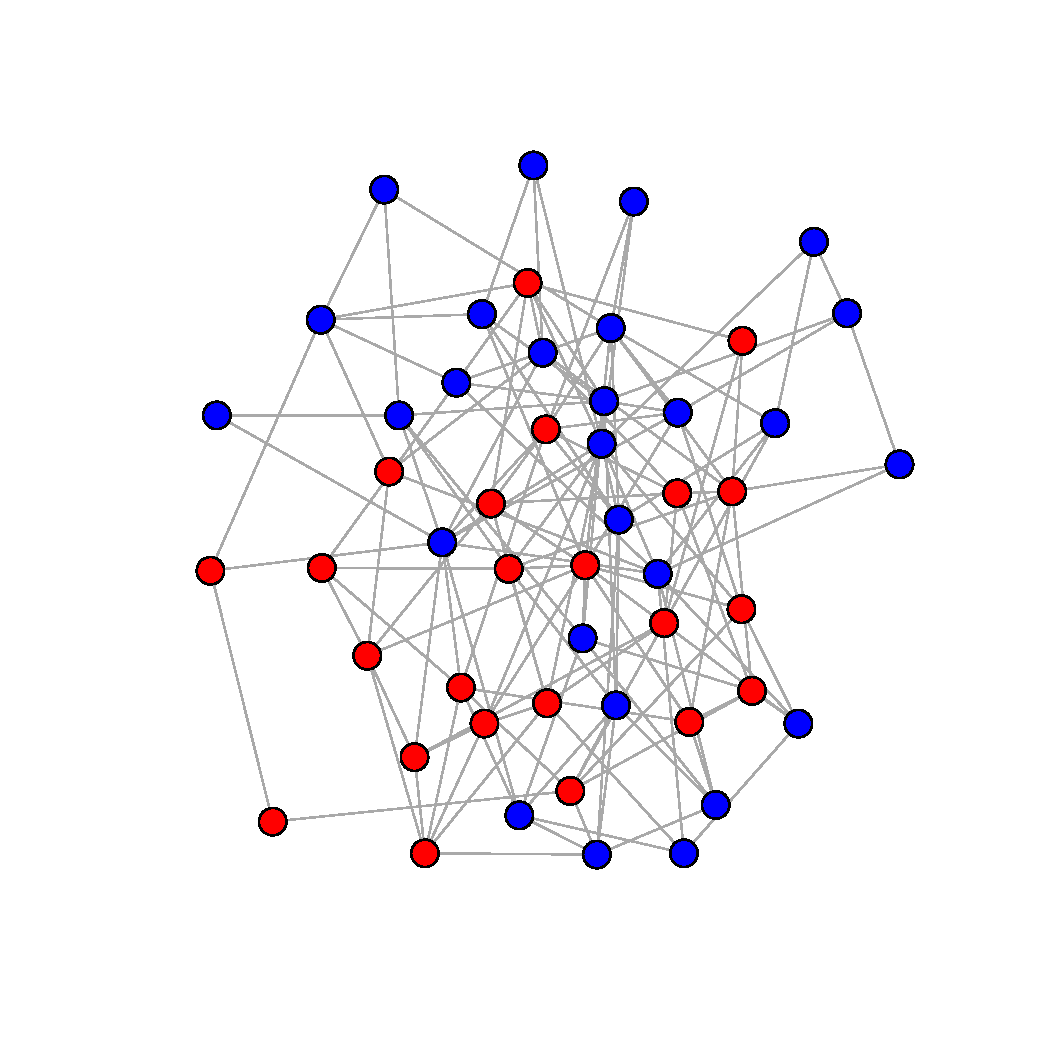
\includegraphics[width = 1in, height = 1in]{g2_beamer.pdf}};
    \node[shape=rectangle, align = center] (Gm) at (-4,-2.5) {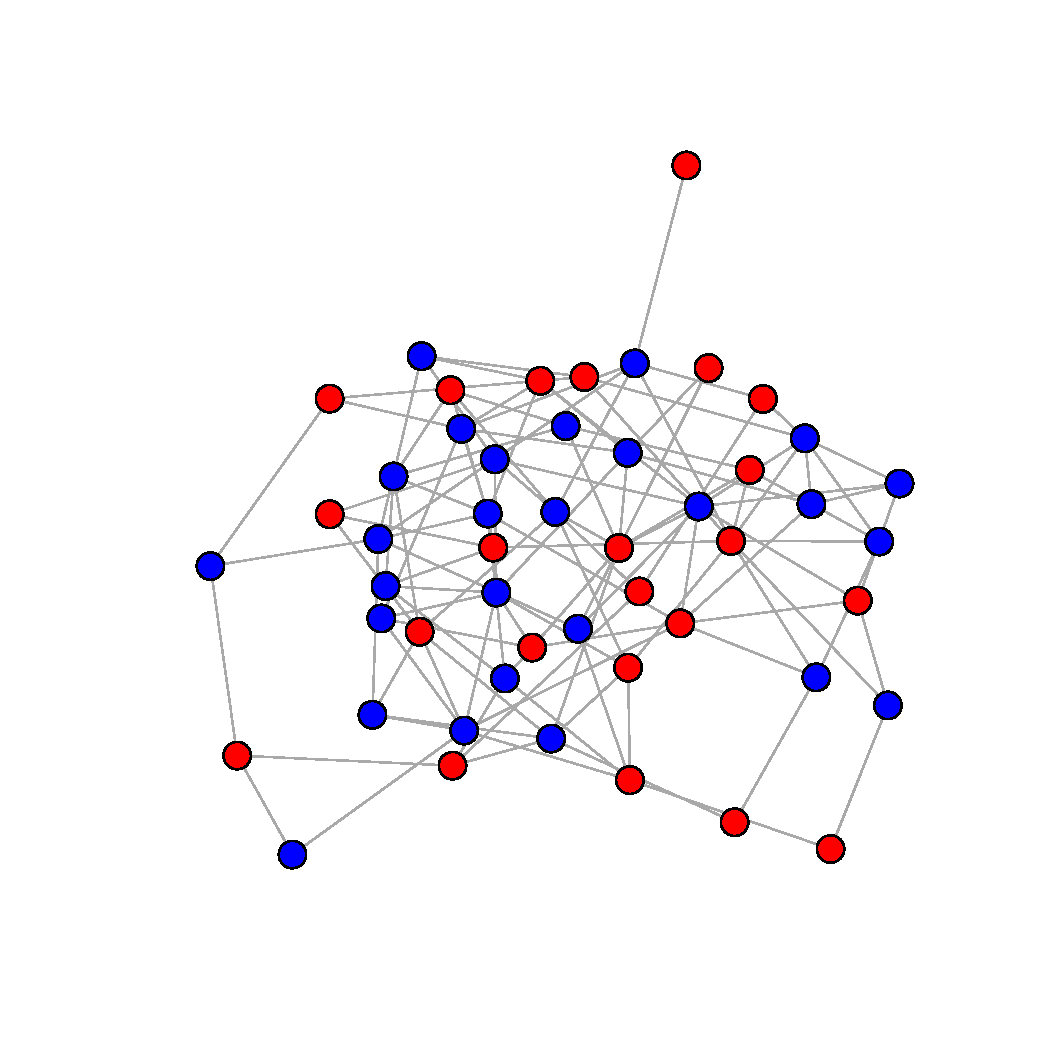
\includegraphics[width = 1in, height = 1in]{g3_beamer.pdf}};
    
    %Draw Adjacency Matrices
    \node[shape=rectangle, align = center] (A1) at (-2,2.5) {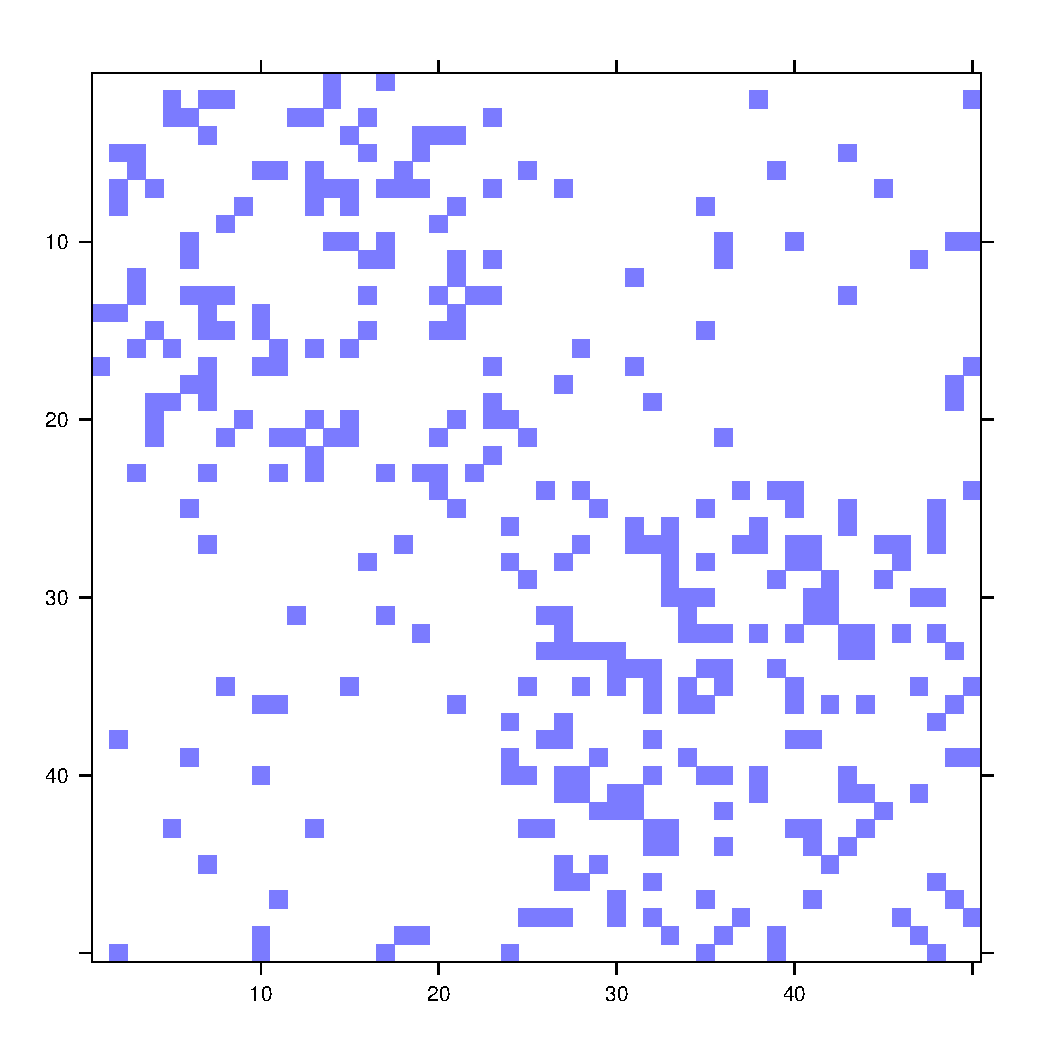
\includegraphics[width = .7in, height = .7in]{A1_beamer.pdf}};
    \node[shape=rectangle, align = center] (Ag) at (-2,0) {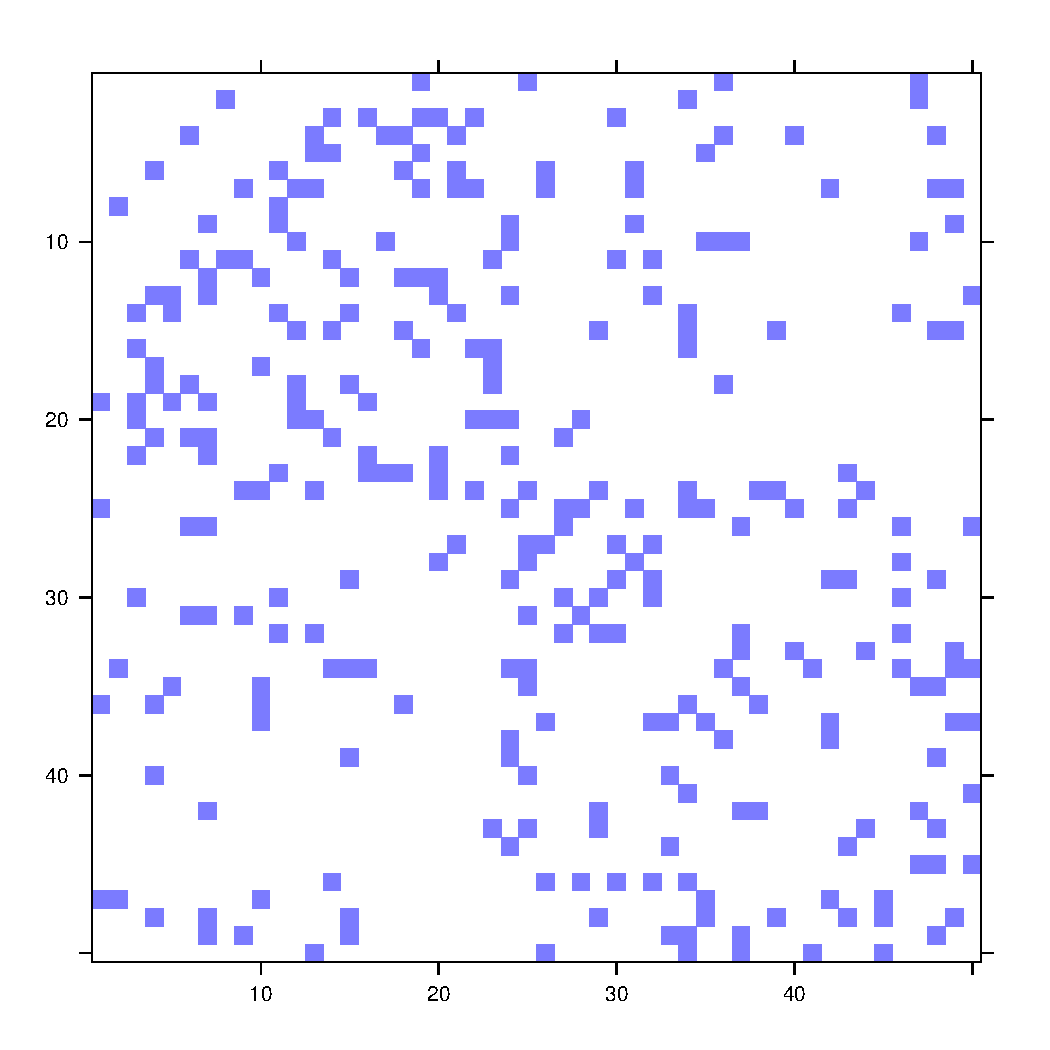
\includegraphics[width = .7in, height = .7in]{A2_beamer.pdf}};
    \node[shape=rectangle, align = center] (Am) at (-2,-2.5) {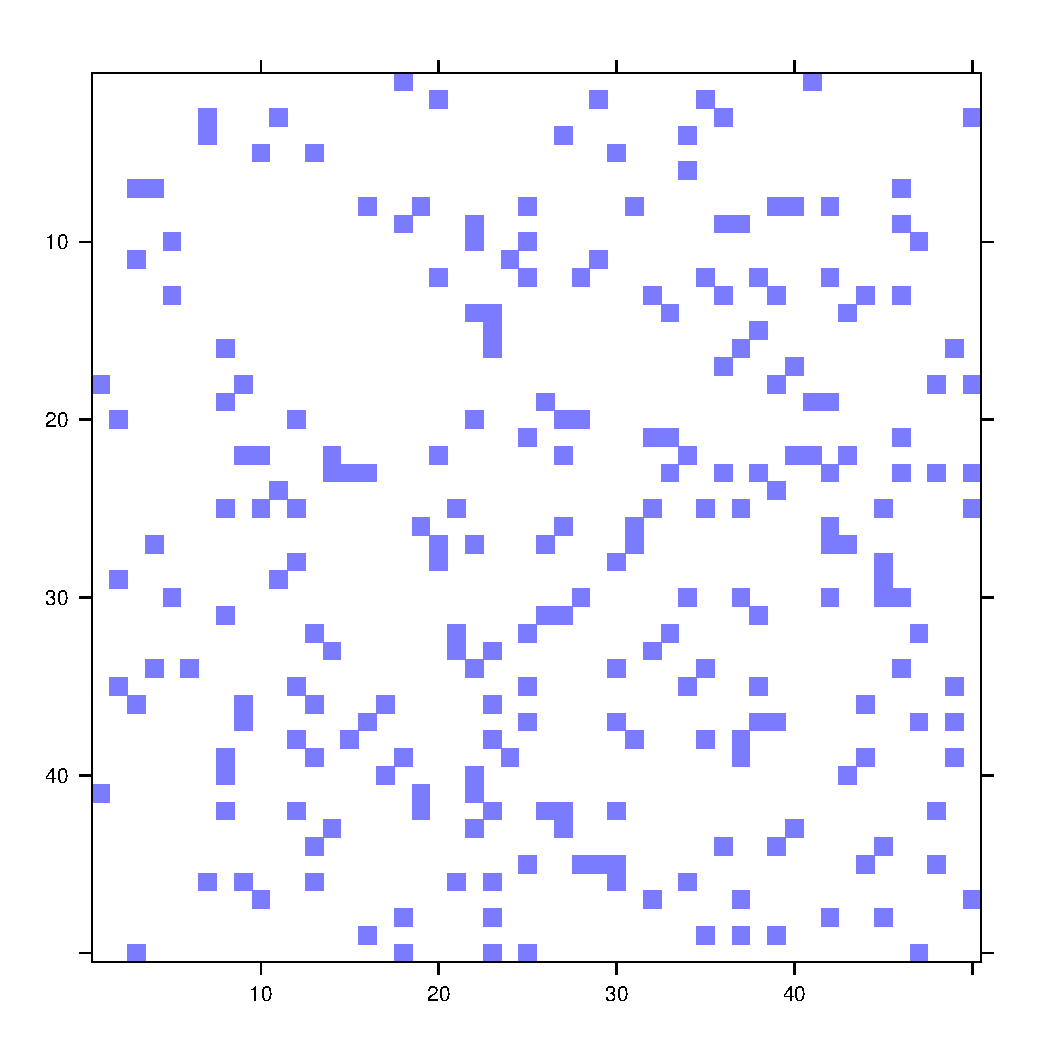
\includegraphics[width = .7in, height = .7in]{A3_beamer.pdf}};
    \pause
    
    %Draw Omni
    \node[shape=rectangle, align = center, draw = black, text width = 1.5cm] (Omni) at (0.5, 0){\scriptsize{Omnibus Embedding}};
    
    
    %Draw arrows
    %\draw (A1)--(-.4,.5); \draw[->] (1.4, 0.5)--(E1);
    %\draw (Ag)--(-.4, 0); \draw[->] (1.4, 0)--(Eg);
    %\draw (Am)--(-.4,-.5); \draw[->] (1.4, -0.5)--(Em);
    
    \draw (A1)--(-.4,0); \draw[->] (1.4, .2)--(E1);
    \draw (Ag)--(-.4, 0); \draw[->] (1.4, 0)--(Eg);
    \draw (Am)--(-.4,0); \draw[->] (1.4, -.2)--(Em);

    %Draw Omni
    \node[shape=rectangle, align = center] (E1) at (3,2.5) {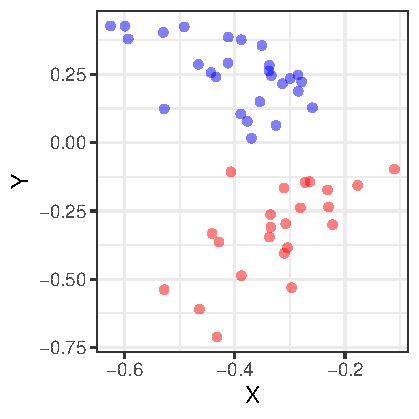
\includegraphics[width = .8in, height = .8in]{embedded_points_0_three_vals.pdf}};
    \node[shape=rectangle, align = center] (Eg) at (3,0) {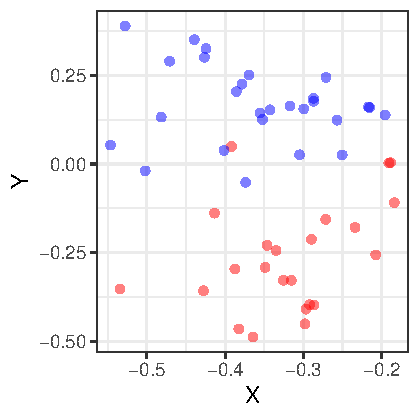
\includegraphics[width = 0.8in, height = .8in]{embedded_points_5_three_vals.pdf}};
    \node[shape=rectangle, align = center] (Em) at (3,-2.5) {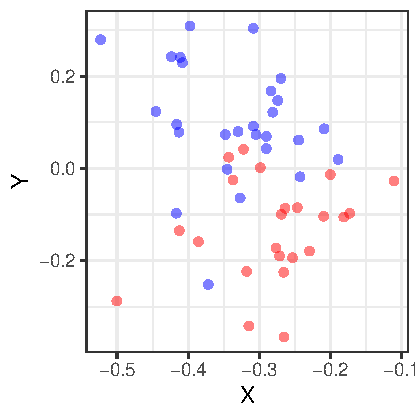
\includegraphics[width = 0.8in, height = .8in]{embedded_points_1_three_vals.pdf}};\pause
    
    
    %draw bracket 
    \draw [decorate, decoration={brace,amplitude=10pt,raise=4pt}]
(4,3.5) -- (4,-3.5) node [black,midway,xshift=1.25cm,text width=1.5cm] {\footnotesize{Statistical Inference}};\pause

    %Draw Omni
    \node[shape=rectangle, align = center, draw = yellow, line width = 1mm, text = black,  text width = 1.5cm] (Omni) at (0.5, 0){\scriptsize{Omnibus Embedding}};
    
\end{tikzpicture}
\end{center}     
\end{frame}


%--------------------------------------------------------------
\section{Bias-Variance Tradeoffs}

\begin{frame}{Network Embedding Techniques}
    \begin{itemize}
        \item ASE, Abar, Omnibus
    \end{itemize}
\end{frame}

\begin{frame}{Estimation Task}
    \begin{itemize}
        \item Introduce ESRDPG
        \item State Estimation task
        \item Plan to compare methods by MSE 
    \end{itemize}

\end{frame}

\begin{frame}{Mean Squared Error Comparison}
    \begin{itemize}
        \item Suppose $\bvar{A}^{(1)}\sim\text{ER}(p)$ and $\bvar{A}^{(2)}\sim\text{ER}(c^2p)$
        \item Under ESRDPG $\bvar{X} = \sqrt{p}\bvar{1}_n$,  $\bvar{C}^{(1)} = \bvar{I}$, and $\bvar{C}^{(2)} = c^2\bvar{I}$
    \end{itemize}\pause
\begin{center}
    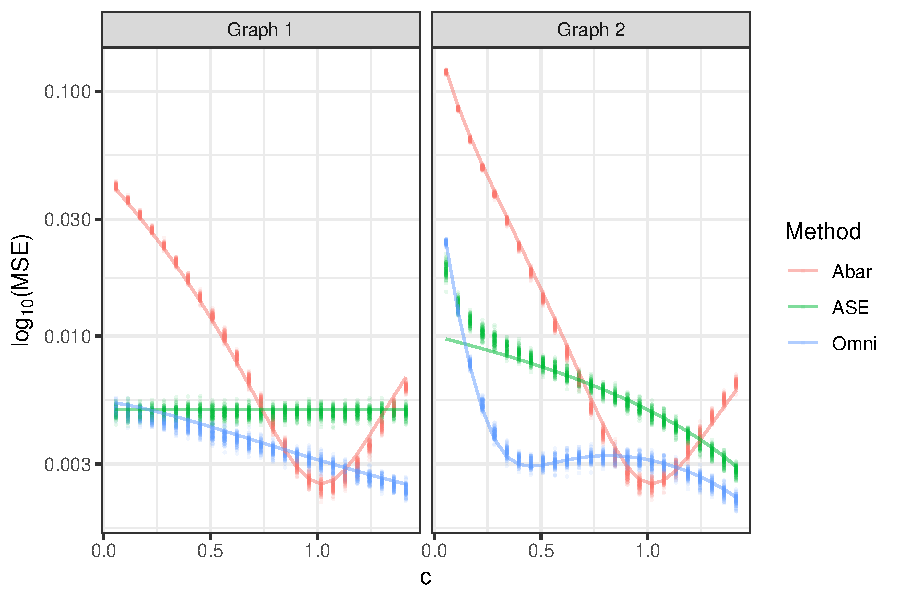
\includegraphics[width = 4in, height = 2.5in]{1d_mse.pdf}
\end{center}
\end{frame}

\begin{frame}{Main Results}
    \begin{itemize}
        \item Asympoptic Expansion 
        \item Theorem Statements 
    \end{itemize}
\end{frame}

%--------------------------------------------------------------
\section{Network Hypothesis Testing}


\begin{frame}{Pivotal Test Statistic}
    \begin{itemize}
        \item Hypotheses, test statistic (both $W$ and $\hat{W}$), approximate asympoptic distribution 
    \end{itemize}
\end{frame}

\begin{frame}{Power Analysis}
    \begin{itemize}
        \item Example, introduction of T statistic, power curves
    \end{itemize}
\end{frame}



\begin{frame}{Conclusion \& Future Work}
    \begin{itemize}
        \item Introduced the \textit{MCRDPG} probability model
        \item Highlighted an advantageous bias-variance tradeoff given by the Omnibus Embedding
        \item Established
        \begin{enumerate}
            \item Bias of the Omnibus Estimator under the \textit{MCRDPG}
            \item Uniform bound on the residual term at a $O(m^{3/2}\log nm/\sqrt{n})$ rate 
        \end{enumerate}
        \item  Highlighted second moment properties of the Omnibus Embedding
    \end{itemize}
    
\end{frame}

\begin{frame}{}
    \begin{center}
        {\Large Questions?}
    \end{center}
\end{frame}

\nocite{*}
\begin{frame}[t,allowframebreaks]
  \frametitle{References}
  \printbibliography
 \end{frame}
%--------------------------------------------------------------







\end{document}


